\section{کار با سنسور \lr{LM35} و استفاده از آن در ساخت فن هوشمند بر اساس دما}

\subsection{اهداف آزمایش}
\begin{itemize}
    \item آشنایی با سنسور دمای \lr{LM35}
    \item آشنایی با نحوه‌ی کار با ترانزیستور برای سوییچینگ و استفاده از منبع تغذیه خارجی
\end{itemize}
\subsection{قطعات مورد نیاز}
\begin{itemize}
    \item بورد \lr{Arduino Uno}
    \item سنسور \lr{LM35}
    \item موتور \lr{DC}
    \item ترانزیستور \lr{BC140}
    \item دیود \lr{1N4001}
    \item منبع تغذیه
    \item مقاومت ۱ کیلواهم
\end{itemize}

\subsection{مقدمه}

\begin{nas} سنسور \lr{LM35} \end{nas}
\newline
\lr{LM35} یک سنسور دمای ولتاژ پایین به درجه سانتی‌گراد است. خروجی این سنسور یک ولتاژ است که به طور خطی با دما به درجه سانتی‌گراد متناسب است و کار با آن بسیار آسان است.
\newline
این سنسور نیازی به کالیبراسیون ندارد و دقت آن ۱ درجه سانتی‌گراد در محدوده دمایی -۵۵ تا +۱۵۵ است. این سنسور می‌تواند با منبع تغذیه ۴ تا ۳۰ ولت تغذیه شود و مصرف جریانی کمتر از ۶۰ میکروآمپر دارد.
\newline
\lr{LM35} در سه شکل مختلف عرضه می‌شود اما رایج ترین نوع آن بسته ۳ پین است که شکلی مشابه یک ترانزیستور دارد.

\newline
\textcolor{red}{\begin{nas}سوال: \end{nas}}
در رابطه با پایه های سنسور \lr{LM35} تحقیق کرده و وظیفه و محدوده ولتاژ ورودی و خروجی قابل قبول هر پایه را بنویسید. برای این کار می‌توانید به دیتاشیت این سنسور مراجعه کنید. محدودی های ولتاژی و جریانی معمولا در قسمتی از دیتاشیت به اسم \lr{Electrical Characteristics} قرار دارند.
\newline

پایه خروجی \lr{LM35} به یکی از ورودی های آنالوگ آردوینو متصل می‌شود. مقدار این ورودی را می‌تواند با تابع \lr{analogRead} خواند.
\newline
\textcolor{red}{\begin{nas}سوال: \end{nas}}
در رابطه با تابع \lr{analogRead} تحقیق کنید و در مورد ورودی و خروجی این تابع توضیح دهید. خروجی این تابع چیست و در چه محدوده‌ای قرار دارد؟
\newline

برای تبدیل خروجی تابع \lr{analogRead} به مقدار دمایی که سنسور به ما می‌دهد باید ابتدا این خروجی را به مقدار بین ۰ تا ۵ ولت تبدیل کرده و سپس آن را ضرب در ۱۰۰ کنید.
\newline
\textcolor{red}{\begin{nas}سوال: \end{nas}}
شبه کد تبدیل خروجی \lr{analogRead} به دما را بنویسید.

\newline
\begin{nas}ترانزیستور\end{nas}
\newline
آردوینو تنها می تواند ۴۰ میلی آمپر در ولتاژ ۵ ولت را روی پین های دیجیتال خود ارائه دهد. اکثر موتورها برای کار کردن به جریان ویا ولتاژ بیشتری نیاز دارند. یک ترانزیستور می تواند به عنوان یک سوئیچ دیجیتال عمل کند و آردوینو را قادر می سازد تا بارهای با نیازهای الکتریکی بالاتر را کنترل کند. به این صورت که ما از پین خروجی آردوینو صرفا برای خاموش و روشن کردن کلید استفاده می‌کنیم و جریان تغذیه اصلی را از یک منبع تغذیه خارجی می‌گیریم.
\newline
ترانزیستور ها دارای سه پایه هستند. در ترانزیستور های پیوندی دوقطبی یا \lr{Bipolar Junction Transistor} این پایه ها بیس، امیتر و کلکتور نام دارند. نحوه‌ی کار آنها به زبان ساده به این صورت است که عبور جریانی کوچک در پایه‌ بیس باعث این می‌شود که جریانی بسیار بزرگ‌تر از پایه کلکتور به امیتر برود. این ترانزیستور ها در دو نوع \lr{pnp} و \lr{npn} وجود دارند که اشاره به ساختار داخلی آن دارند.
\newline
توجه کنید که به دلیل ساختار داخلی ترانزیستور های دوقطبی جهت جریان عبوری بین پایه های امیتر و کلکتور مهم است. به اسم پایه ها توجه کنید، پایه امیتر همانطور که از اسمش پیداست وظیفه تزریق حامل بار و پایه کلکتور وظیفه‌ی جمع‌آوری آنها را دارد. در ترانزیستور های \lr{npn} حامل بار الکترون است پس جهت الکترون ها از امیتر به کلکتور و جهت جریان از کلکتور به امیتر است. در ترانزیستور های \lr{pnp} اما برعکس این است و جریان از امیتر به کلکتور است.
در قرار دادن ترانزیستور در مدار حتما به این نکته توجه کنید.
\newline
\textcolor{red}{\begin{nas}سوال: \end{nas}}
با توجه به نکته‌ای که گفته شد، در هر کدام از ترانزیستور های \lr{npn} و \lr{pnp} مشخص کنید که کدام یک از پایه های امیتر و کلکتور به موتور و منبع تغذیه متصل می‌شوند.

\newline
\begin{nas}موتور \lr{DC}\end{nas}
\newline
موتورهای \lr{DC} از طریق القای مغناطیسی کار می‌کنند. هنگامی که جریان وارد سیم یک میدان مغناطیسی ایجاد می‌شود. با افزایش جریان میدان مغناطیسی قوی‌تر شده و ارتباط این میدان مغناطیسی با آهن ربا های داخل موتور سبب چرخیده شدن شفت مرکزی موتور می‌شود. برعکس این عملیات نیز صادق است، یعنی با چرخاندن موتور می‌توانیم تولید جریان کنیم. به همین دلیل باید در مدار یک دیود نیز قرار دهیم تا در صورتی که موتور ما به هر دلیلی تولید جریان کرد از عبور این جریان جلوگیری شده تا باعث آسیب رساندن به قطعات نشود.

\subsection{شرح آزمایش}
\begin{enumerate}
    \item در هیچکدام از مراحل گفته شده قبل از دو مرحله آخر آردوینو متصل به برق و روشن نباشد.
    \item منبع تغذیه را روشن کنید و مقدار خروجی آن را روی ۵ ولت تنظیم کنید.
    \item سنسور را به آردوینو متصل کنید. برای این کار به شکل پایه‌های سنسور نگاه کنید.
    پین های \lr{4-20V} و \lr{GND} به ترتیب به مثبت و منفی منبع تغذیه متصل میشود و پایه \lr{OUT} نیز به یکی از پین های آنالوگ آردوینو. پین های آنالوگ آردوینو آن‌هایی هستند که شماره آنها با حرف \lr{A} شروع می‌شود.
    \item ممکن است به دلایل مختلف سیگنال خروجی سنسور مشکل دار باشد. خروجی سنسور را به اسیلوسکوپ وصل کنید. با استفاده از کنترل مربوط به \lr{DIV/VOLT} اندازه‌ی موج نمایش داده شده را تغییر دهید تا به حد مناسبی برسد.
    \item اگر شکل موج ثابت بود خروجی شما درست است، اما اگر موج دندانه اره‌ای داشتید خروجی مشکل دارد. سعی کنید با جابجا کردن سنسور در بردبورد این مشکل را رفع کنید.
    \item ولتاژ خروجی سنسور را از اسیلوسکوپ را مشاهده کنید و آن را ضرب در ۱۰۰ کنید. عددی که دارید چه چیزی را نشان می‌دهد؟
    \item مدار مربوط به موتور را ببندید. ابتدا برای آسیب نرسیدن به بورد بر اثر جریان های بازگشتی یک دیود در جهت منفی به مثبت موتور قرار دهید. توجه کنید که جهت مثبت و منفی موتور را خودتان تعیین می‌کنید و با تعویض آن صرفا جهت چرخیدن موتور تغییر می‌کند.
    \item ترانزیستوری که در آزمایشگاه استفاده می‌کنید یک ترانزیستور \lr{NPN} است. این یعنی باید پایه کلکتور به مثبت منبع تغذیه وصل شود.
    \item پایه‌ی امیتر را به مثبت موتور وصل کنید و منفی موتور را به زمین وصل کنید.
    \item پایه بیس را ابتدا به مقاومت ۱ کیلواهمی و سپس به یکی از پین های آردوینو وصل کنید.
    \item برنامه شما باید به گونه‌ای باشد که هر ۵۰۰ میلی‌ثانیه اطلاعات را از سنسور بگیرد و اگر دما از حد آستانه‌ی ۳۰ درجه بیشتر بود، موتور را روشن کند.
    \item برای برنامه ریزی آردوینو، ابتدا تمام اتصالات به پین های آردوینو را جدا کرده و سپس با استفاده از \lr{USB} آن را پروگرام کنید.
    \item برای اجرای برنامه تان، بعد از قطع کردن اتصال \lr{USB}، مثبت منبع تغذیه را به پین \lr{VIN} و منفی منبع تغذیه را به پین \lr{GND} آردوینو متصل کنید.
\end{enumerate}

\newline
\begin{figure}[h]
    \centering
    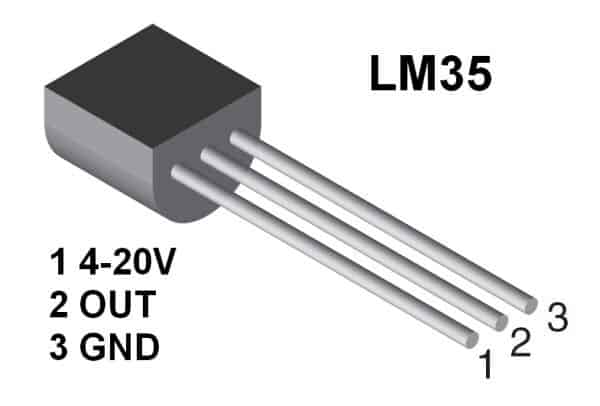
\includegraphics[width=8cm]{lm35.png}
    \caption{پین های سنسور}
    \label{fig:lm35}
\end{figure}
\newline

\newline
\begin{figure}[h]
    \centering
    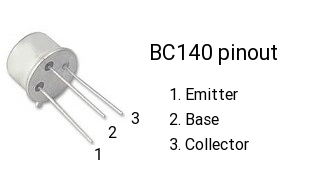
\includegraphics[width=8cm]{bc140.png}
    \caption{پین های ترانزیستور. زائده‌ای که روی ترانزیستور قرار دارد جهت پایه امیتر را نشان می‌دهد.}
    \label{fig:lm35}
\end{figure}
\newline

\newline
\begin{figure}[h]
    \centering
    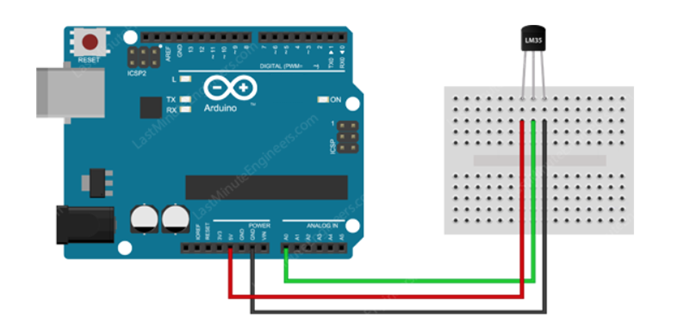
\includegraphics[width=8cm]{l5_c1.png}
    \caption{مدار اتصال سنسور به تنهایی}
    \label{fig:l5-c2}
\end{figure}
\newline

\newline
\begin{figure}[h]
    \centering
    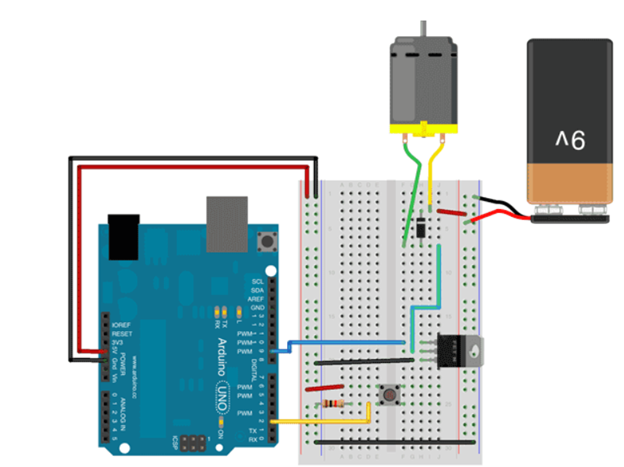
\includegraphics[width=8cm]{l5-c2.png}
    \caption{مدار اتصال موتور. توجه داشته باشید که به جای باطری از منبع تغذیه استفاده می‌کنیم و مقاومت پایه‌ بیس در شکل نیامده. به هیچ عنوان بدون مقاومت متصل به پایه بیس ترانزیستور مدار را روشن نکنید.}
    \label{fig:l5-c2}
\end{figure}
\newline